\chapter{A Case Study of Direct Deep Reinforcement Learning of Decision Tree Policies}
In this chapter compare direct reinforcement learning of decision tree policies to imitation learning (cite) of decision tree policies.
We follow the methodology introduced in (cite) and summarized in Figure (cite) to learn decision tree policies for the CartPole control problem.
In particular, we attempt to reproduce the results from Table (cite) in which authors use imitation learning or deep reinforcement learning in IBMDPs to directly learn a detph-2 decision tree for the CartPole control.

We run the \textit{same} algorithms using the \textit{same} hyperparameters when possible and show our results differ from (cite) in that we find that direct interpretable reinforcement learning underperforms compared to the indirect approach (cite).

\section{Reproducing ``Iterative Bounding MDPs: Learning Interpretable Policies via Non-Interpretable Methods''}

\subsection{IBMDP formulation}
As described in (cite), given a base MDP $\mathcal{M}\langle S, A, R, T, T_0\rangle$, in order to define an IBMDP $\mathcal{M}_{IB}\langle S\times O, A\cup A_{\info}, (R, \zeta),( T, T_0, T_{info})\rangle$, the user needs to provide the set of information gathering actions $A_{info}$ and the reward $\zeta$ for taking those.

For CartPole and other MDPs with large state spaces, authors propose to parametrize the set of IGAs with $i \times p$ actions $\langle v_k, i \rangle$ with $v_k$ depending on the current observation $\boldsymbol{o}_t=(L'_1, U'_1, \dots, L'_i, U'_i, \dots, L'_n, U'_n)$: $v_k = \frac{k(U'_i - L'_i)}{p+1}$.
This parametric IGAs space keeps the discrete IBMDP action space at a reasonable size while providing a learning agent with very veried tests.

For example, if we define an IBMDP with $p=3$ for the grid world IBMDP from Example (cite), at every time six actions are available. 
At $t=0$, recall that $\boldsymbol{o}_0=(0, 2, 0, 2)$, so if an agent takes, e.g., IGA $\langle v_2, 2 \rangle$, the effective IGA is $\langle v_2=\frac{k(2-0)}{3+1}, i \rangle = \langle 1, 2 \rangle$ which in turn effectively corresponds to an internal decision tree node $y \leq 1$.
If the current state $y$-feature value is $0.5$, then the next observation at $t=1$ is $\boldsymbol{o}_1=(0, 2, 0, 1)$. At $t=2$ if $a_t=\langle v_2, 2 \rangle$ again, it would be effectively $\langle v_2=\frac{k(1-0)}{3+1}, i \rangle = \langle 0.5, 2 \rangle$. 
This would give the next observation at $t=2$ $\boldsymbol{o}_2=(0, 2, 0, 0.5)$ and so on \dots. 

Furthermore, author propose to regularize the learned decision tree policy with a maximum depth parameter $D$.
Unfortunately, authors did not describe how they implemented the depth control in their work, hence we have to try different approaches to reproduce their results.

To control the tree depth during learning we can either give negative reward for taking $D$ IGAs since the last base action, or we could terminate the trajectory. 
The penalization approaches can break the MDP formalism because the reward function now depends on time while it should only depend on states and actions (cite). 
Similarly, the termination approach requires a transition function that depends on time breaking the Makrov property.

We actually find that when $p+1$, the IBMDP information gathering space parameter, is a prime number, then as a direct consequence of the \textit{Chinese Reminder Theorem} (cite)(proof), the current tree depth is directly encoded in the current observation $o_t$. 
Hence, when $p+1$ is prime, we can control the depth through trnasitions or rewards without tracking the time.

We will try various $\zeta$, various $p$ and various depth control approaches in our experiments but first we describe the reinforcement learning agents.


\subsection{Modified Deep Reinforcement Learning algorithms}
Authors of (cite) use two deep reinforcement learning baselines to which they apply some modifications in order to learn partially observable policies as required by proposition (cite).

The first algorithm is a modified proximal policy optimization algorithm (PPO)(cite)(algo).
To satisfy proposition (cite) authors modify the default PPO and train a neural network policy $O\rightarrow A\cup A_{info}$ while the neural network value function is $S\times O\rightarrow A\cup A_{info}$ like in the traditional PPO.

The second deep reinforcement learning algorithm used is the deep Q-networks algorithm (DQN) (cite)(algo).
A similar modification is done to DQN to work with partially observable policy. The trained $Q$-function is approximated with a neural network $O\rightarrow \rightarrow \mathbb{R}^{|A\cup A_{info}|}$ rather than $S\times O\rightarrow \mathbb{R}^{|A\cup A_{info}|}$.
In this modified DQN, the temporal difference error target for the $Q$-function $O\rightarrow A\cup A_{info}$ is approximated by a neural network $S\times O\rightarrow A\cup A_{info}$ that is in turn trained by bootstrapping the temporal difference error with itself.

Those two variants of DQN and PPO have first been introduced in (PINTO) for robotics task and later studied theoretically to solve POMDPs (cite) in Baisero's work and we defer their connexions to direct interpretable reinforcement learning to the next Chapter.

Next, we present the precise experimental setup we use to reproduce the work of (cite) in order to study direct deep reinforcement learning of decision tree policies for the CartPole MDP.

\section{Experimental setup}
\subsection{(IB)MDP} 

We use the exact same MDP and associated IBMDP for our experiments as authors of (cite) except mentioned otherwise.

\paragraph{MDP} The problem at hand is the CartPole MDP. At each time step a learning agent observes the cart position velocity and the pole angle and angular velocity, and can take action to push the cart left or right. While the cart is roughly balanced, i.e., while the cart angle remains in some fixed range, the agent gets a positive reward.
If the cart is out of balance; the agent goes to an absorbing terminal state and gets 0 reward forever.
In practice, authors use the gymnasium \texttt{CartPole-v0} implementation (cite) of the CartPole MDP in which trajectories are truncated after 200 timesteps making the maximum cumulative reward over a trajectory to be 200.
Since the IBMDP definition requires the MDP state space to be a factor of bounded segments, authors bound the the state space of the CartPole MDP to be in $[-2, 2] \times [-2, 2] \times [-0.14, 0.14] \times [-1.4, 1.4]$.

\paragraph{IBMDP} Authors define the associated IBMDP with $\zeta=-0.01$ and parametric information gathering action space defined by $p=3$.
In addition we also try $\zeta=0.01$ and $p=2$.
The discount factor used by the authors is $\gamma=1$.

We potentially differ from the original paper setting in the way we handle maximum depth limiation. 
Indeed authors restrain the learning of policies to be equivalent to depth-2 trees but don't detail how they do so.
We hence try two different approaches as mentioned in the previous secion: terminating trajectories if the agent takes too much information gathering in a row or simply giving a reward of $-1$ to the agent everytime it takes an information gathering action past the depth limit.
We will also try IBMDPs where we do not limit the maximum depth for completeness.

\subsection{Baselines}
\paragraph{Modified DQN} as mentioned above, authors use a modified version (cite) of the DQN algorithm (cite).
We use the exact same hyperparameters for Modified DQN as the authors when possible. 
We use the same layers width (128) and number of hidden layers (2), the same exploration strategy ($\epsilon$-greedy with linarly decreasing value $\epsilon$ between 0.5 and 0.05 during the first 10\% of the training),
the same replay buffer size ($10^6$) and the same number of transitions to be collected randomly before doing value updates ($10^5$).
We also try to use more exploartion during training (change the initial $\epsilon$ value to 0.9).
We use the same optimizer (RMSprop (cite) with hyperparmeter 0.95 and learning rate $2.5 \times 10^{-4}$) to update the $Q$-networks.

Authors did not share what DQN implementation they used so we use the stable-baselines3 one (cite).
Authors did not share what activations they used so we try both $\operatorname{tanh}()$ and $\operatorname{relu}()$. 

\paragraph{Modified PPO} for the modified PPO algorithm, we can exactly match the authors hyperparameters since they use the open source stable-baselines3 implementation of PPO.

Similarly to authors of (cite) we train Modified DQN on 1 million timesteps and Modified PPO on 4 million timesteps.

\paragraph{DQN and PPO} We also benchmark the non-modified standard DQN and PPO when learning fully observable IBMDP policies $\pi:S\times O\rightarrow A\cup A_{info}$ and when learning standard $\pi:S\rightarrow A$ policies directly in the CartPole MDP.

We summarize hyperpameters for the IBMDP and for the learning algorithms in Tables (cite) and (cite).

\begin{table}[h]
    \centering
    \caption{IBMDP hyperparameters. We try 12 different IBMDPs. In \textcolor{green}{green} we highlight the hyperparameters from the original paper and in \textcolor{red}{red} we highlight the hyperparameter names for which author do not give information.}
    \begin{tabular}{ll}
    \toprule
    \textbf{Hyperparameter} & \textbf{Values}\\
    \midrule
    Discount factor $\gamma$ & \textcolor{green}{1} \\
    Information gathering actions parameter $p$ & 2, \textcolor{green}{3} \\
    Information gathering actions rewards $\zeta$ & \textcolor{green}{-0.01}, 0.01 \\
    \textcolor{red}{Depth control} & Done signal, negative reward, none \\ 
    \bottomrule
    \end{tabular}
    \end{table}

\begin{table}[h]
    \centering
    \caption{(Modified) DQN trained on $10^6$ timesteps. This gives four different instantiation of (modified) DQN. Hyperparameters not mentioned are stable-baselines3 default. In \textcolor{green}{green} we highlight the hyperparameters from the original paper and in \textcolor{red}{red} we highlight the hyperparameter names for which author do not give information.}
    \begin{tabular}{ll}
    \toprule
    \textbf{Hyperparameter} & \textbf{Values}\\
    \midrule
    Buffer size & \textcolor{green}{$10^6$} \\
    Random transitions before learning & \textcolor{green}{$10^5$} \\
    Epsilon stard & 0.9, \textcolor{green}{0.5} \\
    Epsilon end & \textcolor{green}{0.05} \\
    Exploration fraction & \textcolor{green}{0.1} \\
    Optimizer & \textcolor{green}{RMSprop ($\alpha = 0.95$)}\\
    Learning rate & \textcolor{green}{$2.5\times10^{-4}$}\\
    Networks architectures & \textcolor{green}{[128, 128]}\\
    \textcolor{red}{Networks activation} & $\operatorname{tanh()}$, $\operatorname{relu()}$\\
    \bottomrule
    \end{tabular}
    \end{table}

\begin{table}[h]
    \centering
    \caption{(Modified) PPO trained on $4\times10^6$ timesteps. This gives two different instantiation of (modified) PPO. Hyperparameters not mentioned are stable-baselines3 default. In \textcolor{green}{green} we highlight the hyperparameters from the original paper and in \textcolor{red}{red} we highlight the hyperparameter names for which author do not give information.}
    \begin{tabular}{ll}
    \toprule
    \textbf{Hyperparameter} & \textbf{Values}\\
    \midrule
    Steps between each policy gradient steps & \textcolor{green}{512} \\
    Number of minibatch for policy gradient updates & \textcolor{green}{4} \\
    Networks architectures & \textcolor{green}{[64, 64]}\\
    \textcolor{red}{Networks activations} & $\operatorname{tanh()}$, $\operatorname{relu()}$\\
    \bottomrule
    \end{tabular}
    \end{table}


\paragraph{Indirect methods} We also compare Modified RL algorithm to imitation learning.
To do so, we use Viper or Dagger (cite) to imitate greedy neural network policies obtained with standard DQN learning directly on CartPole.
And we use Dagger to imitate neural network policies obtained with the standard PPO learning directly on CartPole. 

For each indirect method, we imitate the neural network experts by fitting decision trees on 10000 expert transitions using the greedy tree classifier from scikit-learn with default hyperparameters and maximum depth of 2.
    

\subsection{Metrics}
The key metric of this section is performance when controlling the CartPole, i.e, the average undiscounted cumulative reward of a policy on 100 trajectories.

For Modified RL algorithms that learn a partially observable policy (or $Q$-function) in an IBMPD, we periodically extract the policy (or $Q$-function) and use Alg 6 (cite) to extract a decision tree for the CartPole MDP. 
We then evaluate the tree on 100 independent trajectories in the MDP and report the mean undiscounted cumulative reward.

For standard RL applied to IBMDPs, since we can't deploy learned policies directly to the base MDP as the state dimensions mismatch, we periodically evaluate those fully observable IBMDP policies periodically in a copy of the training IBMDP in which we fix $\zeta=0$ ensuring that the cumulative copied IBMDP reward only corresponds to rewards from the base CartPole MDP.
Similarly, we do 100 trajectories of the extracted policies in the copied IBMDP and report the average cumulative reward.

For RL applied directly to the base MDP we can just periodically extract the learned policies and evaluate them on 100 trajectories CartPole control trajectories.

Since imitation learning baselines train offline, i.e, on a fixed dataset, their performances cannot be reported on the same axis as RL baselines.
For that reason, during the training of a standard RL baseline, we periodically extract the trained neural policy/$Q$-function that we consider as the expert to imitate.
Those experts are then imitated with Viper or Dagger using 10 000 newly generated transitions and the fitted decision trees are then evaluated on 100 CartPole trajectories.

Every single combination of IBMDP and Modified RL hyperparameters is run 20 times.
For standard RL on either an IBMDP or an MDP with use the paper's original hyperparameters when they were spicified, with depth control using negative rewards, $\operatorname{tanh()}$ activations, and we repeat this training 20 times. 

Next, we present our results and discuss the reproducibility and limitations of the original approach presented in (cite).

\section{Results}

\subsection{How well do Modified Deep RL baselines learn in IBMDPs?}

\begin{figure}
    \centering
    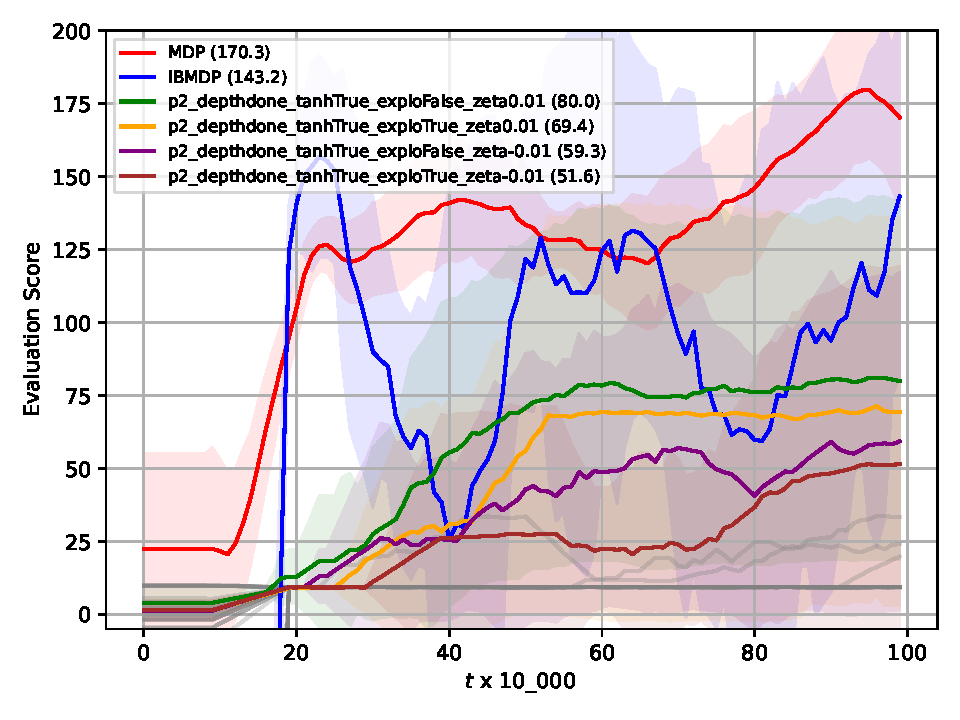
\includegraphics[width=0.8\textwidth]{images/images_part1/dqn.pdf}
    \caption{Variations of Modified DQN, DQN, on CartPole IBMDP variations. We give different line-styles for the learning curves for DQN applied directly on CartPole and DQN applied on the IBMDP.
    Since there are multiple possible candidates for the original paper hyperparametrs, we choose to color the (Modified DQN variant, IBMDP variant) pair that resulted in the best decision tree policy on CartPole among the instances that could match the original paper.
    Shaded areas represent the confidence interval at 95\% at each measure on the y-axis.}
\end{figure}

\begin{figure}
    \centering
    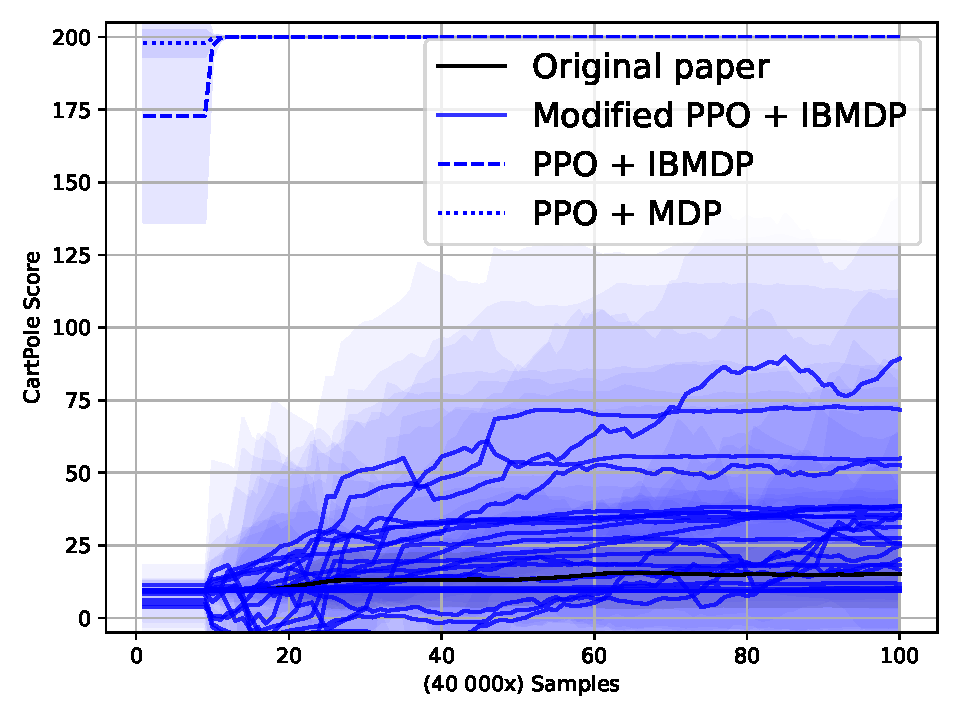
\includegraphics[width=0.8\textwidth]{images/images_part1/ppo.pdf}
    \caption{Variations of Modified PPO, PPO, on CartPole IBMDP variations. We give different line-styles to the learning curves for PPO applied directly on CartPole and PPO applied on the IBMDP.
    Since there are multiple possible candidates for the original paper hyperparametrs, we choose to color the (Modified PPO variant, IBMDP variant) pair that resulted in the best decision tree policy on CartPole among the instances that could match the original paper.
    Shaded areas represent the confidence interval at 95\% measure on the y-axis.}
\end{figure}
On Figure (cite), we observe that Modified DQN can learn in IBMDPs--the curves have an increasing trend--but we also observe that Modified DQN finds poor decision tree policies for CartPole in average--the curves flatten at the end of the x-axis and have low y-values--.
In, particular, among all the learning curves that could possibly correspond to the original paper Modified DQN, the learning curve with highest final y-value is converging to decision tree policies for CartPole high poor performances.

On Figure (cite) we observe that Modified PPO finds decision tree policies with 150 cumulative rewards towrads the end of training. The performance difference with Modified DQN could be because we trained longer, like in the original paper.

However it could also be because DQN-like algorithm with those hyperpameters struggle in general CartPole MDP or IBMDPs.

Indeed, on Figures (cite) and (cite), we observe that baselines seeking fully observable policies (RL + IBMDP and RL + MDP), learn better CartPole policies in average for both DQN and PPO-like baselines. 
We do notice that for DQN-like baselines, learning seems difficult in general indepedently of the setting while on Figure (cite) it is clear that for PPO baselines seeking fully observable, learning is super efficient and agent find optimal policies with reward 200.

In Tables (cite) and (cite) we report the top-5 hyperparameters for Modified RL baselines when learning partially observable IBMDP policies in terms of extracted decision tree policies performances in CartPole control.
\begin{table}[h]
    \centering
    \caption{Top 5 Hyperparameter Configurations for Modified DQN + IBMDP, bold font represent the original paper hyperparameters.}
    \label{tab:top5_results}
    \begin{tabular}{ccccccS}
    \toprule
    Rank & $p$ & Depth control & Activation & Exploration & $\zeta$ & {Final Performance} \\
    \midrule
    1 & 3 & termination & $\operatorname{tanh}()$ & 0.9 & 0.01 & 53 \\
    2 & 2 & termination & $\operatorname{tanh}()$ & 0.5 & -0.01 & 24 \\
    \textbf{3} & \textbf{3} & \textbf{termination} & $\operatorname{tanh}()$ & \textbf{0.5} & \textbf{-0.01} & \textbf{24} \\
    4 & 2 & termination & $\operatorname{tanh}()$ & 0.5 & 0.01 & 23 \\
    5 & 2 & termination & $\operatorname{tanh}()$ & 0.9 & -0.01 & 22 \\
    \bottomrule
    \end{tabular}
    \end{table}

    \begin{table}[h]
        \centering
        \caption{Top 5 Hyperparameter Configurations for Modified PPO + IBMDP, bold font represent the original paper hyperparameters.}
        \label{tab:top5_ppo_results}
        \begin{tabular}{cccccS}
        \toprule
        Rank & $p$ & Depth Control & Activation & $\zeta$ & {Final Performance} \\
        \midrule
        1 & 3 & reward & $\operatorname{relu}()$ & 0.01 & 139 \\
        2 & 3 & done & $\operatorname{relu}()$ & 0.01 & 132 \\
        \textbf{3} & \textbf{3} & \textbf{reward} & $\operatorname{tanh}()$ & \textbf{-0.01} & \textbf{119} \\
        4 & 3 & reward & $\operatorname{relu}()$ & -0.01 & 117 \\
        5 & 3 & reward & $\operatorname{tanh}()$ & 0.01 & 116 \\
        \bottomrule
        \end{tabular}
        \end{table}


\subsection{How does direct interpretable reinforcement learning perform compared to the indirect approach?}

\begin{figure}
    \centering
    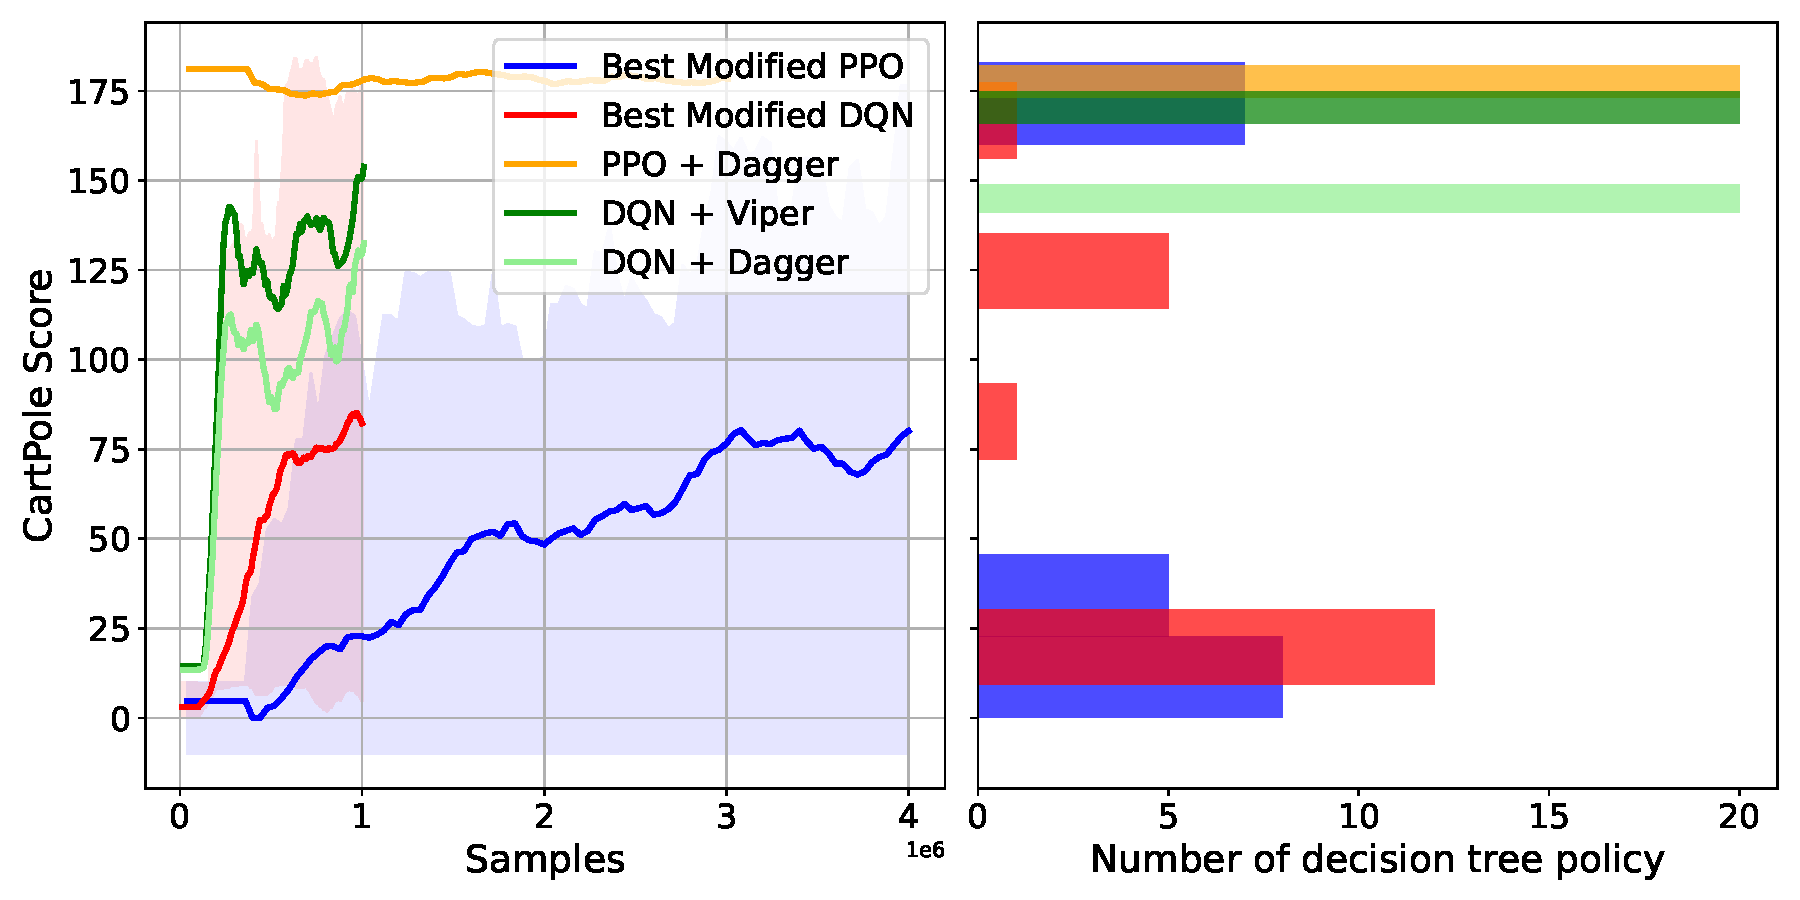
\includegraphics[width=1\textwidth]{images/images_part1/ppo_tree_study.pdf}
    \caption{(left) Mean performance of the best Modified PPO on the best IBMDP with shaded areas representing the min and max performance over the 20 seeds during training. (right) Histogram of the final decision tree policies performances.}
\end{figure}


\begin{figure}[htbp]
    \centering
    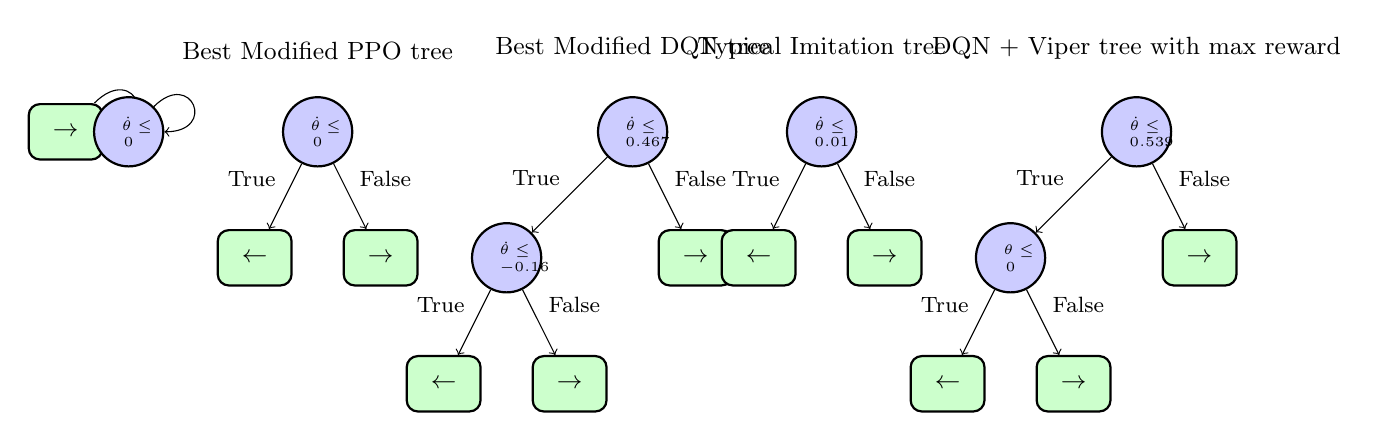
\begin{tikzpicture}[
        scale=0.8,
        decision/.style={circle, draw, thick, fill=blue!20, text width=0.5em, text centered, minimum height=2.5em, font=\tiny},
        leaf/.style={rectangle, draw, thick, fill=green!20, text width=2em, text centered, rounded corners, minimum height=2em, font=\small},
        edge_label/.style={font=\footnotesize, midway}
    ]

        \node[leaf] (tree7_root) at (-4,0) {$\rightarrow$};
        \draw[->] (tree7_root) to[out=45,in=0,looseness=5] (tree7_root);

        \node[decision] (tree7_root) at (-3,0) {$\dot{\theta} \leq 0$};
        \draw[->] (tree7_root) to[out=45,in=0,looseness=5] (tree7_root);
        
        % Tree 4: if x <= 0.5 move right else move left
        \node[decision] (tree4_root) at (0,0) { $\dot{\theta}\leq 0$};
        \node[leaf] (tree4_right) at (-1,-2) {$\leftarrow$};
        \node[leaf] (tree4_left) at (1,-2) {$\rightarrow$};
        \draw[->] (tree4_root) -- (tree4_right) node[edge_label, above left] {True};
        \draw[->] (tree4_root) -- (tree4_left) node[edge_label, above right] {False};
        

        % Tree 7: if x <= 0.5 and y <= 0.5 move right else move down
        \node[decision] (tree7_root) at (5,0) {$\dot{\theta}\leq 0.467$};
        \node[decision] (tree7_y) at (3,-2) {$\dot{\theta}\leq -0.16$};
        \node[leaf] (tree7_right) at (2,-4) {$\leftarrow$};
        \node[leaf] (tree7_down) at (4,-4) {$\rightarrow$};
        \node[leaf] (tree7_down2) at (6,-2) {$\rightarrow$};
        \draw[->] (tree7_root) -- (tree7_y) node[edge_label, above left] {True};
        \draw[->] (tree7_root) -- (tree7_down2) node[edge_label, above right] {False};
        \draw[->] (tree7_y) -- (tree7_right) node[edge_label, above left] {True};
        \draw[->] (tree7_y) -- (tree7_down) node[edge_label, above right] {False};




        % Tree 4: if x <= 0.5 move right else move left
        \node[decision] (tree4_root) at (8,0) { $\dot{\theta}\leq 0.01$};
        \node[leaf] (tree4_right) at (7,-2) {$\leftarrow$};
        \node[leaf] (tree4_left) at (9,-2) {$\rightarrow$};
        \draw[->] (tree4_root) -- (tree4_right) node[edge_label, above left] {True};
        \draw[->] (tree4_root) -- (tree4_left) node[edge_label, above right] {False};


        % Tree 7: if x <= 0.5 and y <= 0.5 move right else move down
        \node[decision] (tree7_root) at (13,0) {$\dot{\theta}\leq 0.539$};
        \node[decision] (tree7_y) at (11,-2) {$\theta\leq 0$};
        \node[leaf] (tree7_right) at (10,-4) {$\leftarrow$};
        \node[leaf] (tree7_down) at (12,-4) {$\rightarrow$};
        \node[leaf] (tree7_down2) at (14,-2) {$\rightarrow$};
        \draw[->] (tree7_root) -- (tree7_y) node[edge_label, above left] {True};
        \draw[->] (tree7_root) -- (tree7_down2) node[edge_label, above right] {False};
        \draw[->] (tree7_y) -- (tree7_right) node[edge_label, above left] {True};
        \draw[->] (tree7_y) -- (tree7_down) node[edge_label, above right] {False};
        


        % Labels
        \node[above] at (0,1) {{\small Best Modified PPO tree}};
        \node[above] at (5,1) {{\small Best Modified DQN tree}};
        \node[above] at (8,1) {{\small Typical Imitation tree}};
        \node[above] at (13,1) {{\small DQN + Viper tree with max reward}};


    \end{tikzpicture}
    \caption{Trees obtained by DRL against trees obtained with imitation.}
    \label{fig:trees-drl}
\end{figure}


On Figure (cite), we isolate the best performing baselines that learn decision tree policies for CartPole using either Modified DQN or Modified PPO and compare them with imitation learning baselines that use the surrogate objective (cite) to find CartPole decision tree policies.
We find that despite having poor performances in \textit{average} (c.f. Figure (cite)), the deep reinforcement learning baselines find very good decision tree policies and also extremly poor ones as shown by the min-max shaded areas on the left of Figure (cite) and the estimated density of final trees performances on Figure (cite).
In fact, when compared with imitation learning baselines, that fit the policy of a PPO + MDP or fit the greedy policy w.r.t to the $Q$-network of a DQN + MDP, when running e.g., 20 seeds of direct reinforcement learning baselines, there are some seeds that can find good decision tree policies as fast as the indirect imitation learning baselines: if we look at the shaded area of Modified DQN on Figure (cite), we can observe that it is consitently overlapping with an inderect method curve.
However this is not desirable, a user want an agent that can consistantly find good decision tree policy.
As shown by the estimated densities (cite), indirect methods consistently find good decision tree policies (the higher modes of distributions are on the right of the plot). On the other hand, the final trees returned by direct RL methods seem equally distributed on both extremes of the scores.

On Figure (cite), we compare the best trees returned by Modified DQN and Modified PPO. We used Algorithm 6 to extract 20 trees from the 20 partially observable policies returned by deeop reinforcement learning over 20 seeds. We then plot the best tree for each baseline. Those trees get an everage reward of roughly 175.
Similarly, we plot a representative tree for imitation learning baseline as well as a tree that has max reward obtained with Viper. 
However unlike for direct methods, the tree returned are extremely similar across seed. In particular they often only vary in the scalar value used in the root node but in general have the same structure and test the angular velocity.
On the other hand the most frequent tree across seed returned by modified RL baselines is the ``infinite'' tree that corresponds to only taking an information gathering action.


\section{Discussion}
We have shown that compared to learning non-interpretable policies for both the base MDP and the associated IBMDP, learning partially observable policies in IBMDP is very difficult even when learning policies corresponding to depth-2 decision trees for the simple CartPole task.
In the next chapter we down scale the learning algorithms to highlight the connexions between the above challenges and POMDP hardness results.